%!TEX program = xelatex
\documentclass[8pt, landscape, a4paper]{extarticle}

% --- 核心宏包 ---
\usepackage[UTF8, fontset=fandol]{ctex}
\usepackage[margin=0.8cm, top=1cm, bottom=1.3cm]{geometry}
\usepackage{multicol}
\usepackage{xcolor}
\usepackage{tcolorbox}
\usepackage{enumitem}
\usepackage{amsmath}
\usepackage{amssymb}
\usepackage{fontspec}
\usepackage{tikz}
\usetikzlibrary{arrows.meta, positioning}

% --- 去掉页码 ---
\pagestyle{empty}

% --- 颜色定义 (紫色主题) ---
\definecolor{headerblue}{RGB}{142, 68, 173}    % 主题紫
\definecolor{navcolor}{RGB}{211, 84, 0}        % 导航橙
\definecolor{intuitioncolor}{RGB}{41, 128, 185}% 直觉蓝
\definecolor{accentcolor}{RGB}{192, 57, 43}    % 强调红
\definecolor{dividergray}{RGB}{220, 220, 220}

% --- 全局设置 ---
\setlength{\parindent}{0pt}
\setlength{\columnsep}{0.4cm} 
\linespread{1.1} 

% --- 列表样式 ---
\setlist[itemize]{leftmargin=1.2em, nosep, itemsep=2pt, topsep=2pt, label=$\textcolor{headerblue}{\vcenter{\hbox{\tiny$\bullet$}}}$ }
\setlist[description]{leftmargin=0.2em, style=sameline, nosep, itemsep=2pt, font=\bfseries}

% --- Box 样式 ---
\newtcolorbox{mybox}[2][]{%
  colback=white,
  colframe=#2,
  coltitle=white,
  boxrule=1pt,             
  arc=2mm,                 
  left=4pt, right=4pt, top=3pt, bottom=3pt, 
  toptitle=3pt, bottomtitle=3pt, 
  fonttitle=\bfseries\sffamily\large,
  title={#1},
  after skip=5pt          
}

% --- 自定义命令 ---
\newcommand{\subt}[1]{{\vspace{2pt}\textbf{\large \textcolor{black}{#1}}}}

\newcommand{\boxdesc}[1]{%
    \textit{\small \textcolor{gray}{#1}}%
    \par\vspace{2pt}%
    {\color{dividergray}\hrule height 0.5pt}%
    \vspace{2pt}%
}

\newcommand{\sepline}{%
    \par \vspace{3pt}%
    {\color{dividergray}\hrule height 0.5pt}%
    \par \vspace{3pt}%
}

% 公式间距
\setlength{\abovedisplayskip}{3pt}
\setlength{\belowdisplayskip}{3pt}

\begin{document}

% --- 页眉 ---
\begin{center}
    {\Huge \textbf{\sffamily \textcolor{headerblue}{概率统计 Probability \& Statistics Cheat Sheet}}} \\
    \vspace{0.2cm}
    {\large \texttt{Managing Uncertainty: From Bayes' Theorem to MCMC}}
\end{center}

% --- 开始四栏布局 ---
\begin{multicols*}{4}

% === 第一栏 (保持 v2.0 内容) ===

\begin{mybox}[��️ 场景导航 (Use Cases)]{navcolor}
    \boxdesc{遇到什么问题 $\to$ 用什么工具}
    \begin{itemize}[itemsep=2pt]
        \item \textbf{垃圾邮件/风控} $\to$ 朴素贝叶斯 (Naive Bayes)
        \item \textbf{流量/排队预测} $\to$ 泊松分布 (Poisson)
        \item \textbf{AB测试/效果评估} $\to$ 假设检验 (P-value)
        \item \textbf{SLA/P99延迟} $\to$ 正态分布/长尾分布
        \item \textbf{复杂系统模拟} $\to$ 蒙特卡洛 (Monte Carlo)
        \item \textbf{模型参数估计} $\to$ MLE / MAP
    \end{itemize}
\end{mybox}

\begin{mybox}[1. 概率公理 (Axioms)]{headerblue}
    \boxdesc{量化不确定性的规则}
    
    \subt{基本公式}
    \begin{itemize}
        \item \textbf{条件概率}: $P(A|B) = \frac{P(AB)}{P(B)}$
        \item \textbf{全概率公式}: $P(A) = \sum P(A|B_i)P(B_i)$
        \item \textbf{独立性}: $P(AB) = P(A)P(B)$
    \end{itemize}
    \sepline

    \subt{贝叶斯定理 (Bayes' Rule)}
    \begin{center}
        {\LARGE \textcolor{accentcolor}{$P(A|B) = \frac{P(B|A)P(A)}{P(B)}$}}
    \end{center}
    \begin{itemize}
        \item \textbf{后验} $\propto$ \textbf{似然} $\times$ \textbf{先验}
        \item \textbf{直觉}: 用新的证据 $B$ 更新对 $A$ 的旧看法。
    \end{itemize}
\end{mybox}

\begin{mybox}[2. 随机变量 (Random Vars)]{headerblue}
    \boxdesc{将事件映射为数字}
    
    \subt{期望与方差}
    \begin{itemize}
        \item \textbf{期望 (Mean)}: $E[X] = \sum x p(x)$ (重心)
        \item \textbf{方差 (Var)}: $Var(X) = E[(X-\mu)^2]$ (波动)
        \item \textbf{协方差}: $Cov(X,Y) = E[(X-\mu_x)(Y-\mu_y)]$
    \end{itemize}
    \sepline
    
    \subt{大数定律 (LLN)}
    样本越多,平均值越接近真实期望。$\bar{X}_n \to \mu$。
    \sepline
    
    \subt{切比雪夫不等式 (Chebyshev)}
    无论分布形状如何,数据偏离均值 $k$ 个 $\sigma$ 的概率:
    $$ P(|X-\mu| \ge k\sigma) \le \frac{1}{k^2} $$
\end{mybox}

\columnbreak

% === 第二栏 (填充+3行) ===

\begin{mybox}[3. 离散分布 (Discrete)]{headerblue}
    \boxdesc{数人头、抛硬币、服务器请求}
    
    \subt{伯努利 (Bernoulli) / 二项 (Binomial)}
    \begin{itemize}
        \item \textbf{场景}: 抛硬币、点击率 (CTR)。
        \item $P(k) = \binom{n}{k} p^k (1-p)^{n-k}$
    \end{itemize}
    \sepline
    
    \subt{泊松分布 (Poisson)}
    $$ P(k) = \frac{\lambda^k e^{-\lambda}}{k!} $$
    \begin{itemize}
        \item \textbf{场景}: 单位时间内到达的请求数、Bug数。
        \item \textbf{特征}: 均值 = 方差 = $\lambda$。事件是独立的。
    \end{itemize}
    \sepline
    
    \subt{几何分布 (Geometric)}
    \begin{itemize}
        \item \textbf{场景}: 第 $k$ 次尝试才成功的概率 (重试机制)。
    \end{itemize}
    \sepline
    
    % 【新增1】多项分布
    \subt{多项分布 (Multinomial)}
    二项分布的推广。$n$ 次试验,$k$ 个类别。
    \textit{场景: NLP 词频统计 (Bag of Words)。}
\end{mybox}

\begin{mybox}[4. 连续分布 (Continuous)]{headerblue}
    \boxdesc{身高、误差、延迟、寿命}
    
    \subt{高斯/正态分布 (Gaussian)}
    $$ f(x) = \frac{1}{\sqrt{2\pi}\sigma} e^{-\frac{(x-\mu)^2}{2\sigma^2}} $$
    \begin{itemize}
        \item \textbf{中心极限定理 (CLT)}: 独立随机变量之和,最终都趋向于正态分布。这是\textbf{误差}通常服从正态分布的原因。
        \item \textbf{法则}: $\pm 1\sigma$ (68\%), $\pm 2\sigma$ (95\%), $\pm 3\sigma$ (99.7\%)。
    \end{itemize}
    \sepline
    


    \subt{指数分布 (Exponential)}
    $f(x) = \lambda e^{-\lambda x}$
    \begin{itemize}
        \item \textbf{场景}: 事件发生的时间间隔、粒子寿命。
        \item \textbf{无记忆性}: 无论等了多久,下一秒发生的概率不变。
    \end{itemize}
    \sepline
    

    
    \subt{对数正态 (Log-Normal)}
    若 $\ln X \sim N(\mu, \sigma^2)$。描述\textbf{乘性误差}累积。
    \textit{场景:用户收入、API 响应延迟 (长尾分布)。}
\end{mybox}

\columnbreak

% === 第三栏 (保持 v2.0 内容) ===

\begin{mybox}[5. 统计推断 (Inference)]{headerblue}
    \boxdesc{从数据反推规律}
    
    \subt{参数估计}
    \begin{itemize}
        \item \textbf{MLE (极大似然)}: 找参数 $\theta$,让数据出现的概率最大。$\max P(D|\theta)$。
        \item \textbf{MAP (最大后验)}: 加上先验知识。$\max P(D|\theta)P(\theta)$。
    \end{itemize}
    \sepline
    
    \subt{假设检验 (Hypothesis Testing)}
    \begin{itemize}
        \item \textbf{H0 (零假设)}: 世界是无聊的 (无效果/无差异)。
        \item \textbf{P-value}: 在 H0 成立下,看到当前数据(或更极端)的概率。P越小,H0越不可信。
        \item \textbf{Type I/II 错误}: 误报 (False Positive) vs 漏报。
    \end{itemize}
    \sepline
    
    \subt{A/B 测试核心}
    双样本均值检验 (T-test / Z-test)。判断两个版本的转化率是否有\textbf{显著差异}。
\end{mybox}

\begin{mybox}[6. 随机过程与 MCMC]{headerblue}
    \boxdesc{动态的随机性}
    
    \subt{马尔可夫链 (Markov Chain)}
    \textbf{无记忆性}: $P(X_{t+1}|X_t, \dots) = P(X_{t+1}|X_t)$。
    \textit{应用: PageRank, 文本生成。}
    \sepline
    
    \subt{蒙特卡洛 (Monte Carlo)}
    用随机采样来解决计算问题 (如求积分、算 $\pi$)。
    \sepline
    
    \subt{MCMC (马尔可夫链蒙特卡洛)}
    构造一个马链,使其平稳分布等于目标分布。
    \begin{itemize}
        \item \textbf{应用}: 贝叶斯推断中,当后验概率 $P(\theta|D)$ 无法直接计算积分时,用 MCMC 采样近似。
    \end{itemize}
\end{mybox}

\begin{mybox}[7. Python / Scipy 实战]{headerblue}
    \boxdesc{代码工具箱}
    \begin{itemize}
        \item \textbf{分布}: \texttt{scipy.stats.norm(loc, scale)}
        \item \textbf{采样}: \texttt{rvs(size=1000)}
        \item \textbf{概率密度}: \texttt{pdf(x)} / \textbf{累积}: \texttt{cdf(x)}
        \item \textbf{检验}: \texttt{ttest\_ind(a, b)}
    \end{itemize}
\end{mybox}

\columnbreak

% === 第四栏 (保持 v2.0 内容) ===

\begin{mybox}[8. 信息论视角 (Information)]{headerblue}
    \boxdesc{概率与编码的桥梁}
    
    \subt{熵 (Entropy)}
    衡量分布的混乱程度/信息量:
    $$ H(X) = - \sum p(x) \log p(x) $$
    \sepline
    
    \subt{KL 散度 (相对熵)}
    衡量两个分布 $P$ 和 $Q$ 的距离:
    $$ D_{KL}(P||Q) = \sum P(x) \log \frac{P(x)}{Q(x)} $$
    \textit{应用: 机器学习中的 Cross-Entropy Loss 就是它。}
    \sepline
    
    \subt{互信息 (Mutual Information)}
    $I(X;Y) = H(X) - H(X|Y)$。
    \textit{含义: 知道 $Y$ 后,消除了多少关于 $X$ 的不确定性。}
\end{mybox}

\vspace*{\fill}

\begin{mybox}[�� 核心直觉 (Intuition)]{intuitioncolor}
    \boxdesc{“世界不是非黑即白,而是灰度的。”}
    
    % TikZ 矢量图
    \begin{center}
    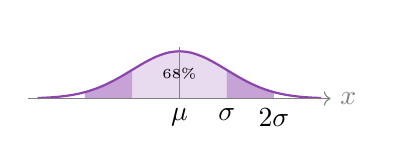
\begin{tikzpicture}[scale=0.6]
        \begin{scope}
            \clip (-3,0) rectangle (3,1.5);
            \fill[headerblue!20] (-1,0) -- plot[domain=-1:1] (\x,{exp(-\x*\x/2)}) -- (1,0) -- cycle;
            \fill[headerblue!50] (-2,0) -- plot[domain=-2:-1] (\x,{exp(-\x*\x/2)}) -- (-1,0) -- cycle;
            \fill[headerblue!50] (1,0) -- plot[domain=1:2] (\x,{exp(-\x*\x/2)}) -- (2,0) -- cycle;
        \end{scope}
        \draw[domain=-3:3, smooth, variable=\x, thick, headerblue] plot ({\x}, {exp(-\x*\x/2)});
        \draw[->, gray] (-3.2,0) -- (3.2,0) node[right] {$x$};
        \draw[gray] (0,0) -- (0,1.1);
        \node[below] at (0,0) {$\mu$};
        \node[below] at (1,0) {$\sigma$};
        \node[below] at (2,0) {$2\sigma$};
        \node[above] at (0,0.2) {\tiny 68\%};
    \end{tikzpicture}
    \end{center}

    \hspace{1em}概率论是程序员处理\textbf{不完全信息}的操作系统。
    \vspace{3pt}
    
    \subt{三大核心视角}
    \begin{itemize}[itemsep=4pt]
        \item \textbf{频率 vs 贝叶斯}: 
        频率派认为参数是固定的 (真理存在);贝叶斯派认为参数也是随机变量 (我们对真理的信心)。大数据时代,贝叶斯思维 (Prior + Data $\to$ Posterior) 更符合 AI 的学习过程。
        
        \item \textbf{分布即形状}: 
        不必死记公式。泊松是“稀疏事件”,高斯是“误差累积”,指数是“无记忆等待”,幂律是“赢家通吃”。看到数据形状,就选什么分布。
        
        \item \textbf{相关 $\neq$ 因果}: 
        统计只能告诉你 A 和 B 同时发生 (Correlation),不能告诉你 A 导致了 B (Causality)。这是数据分析最大的陷阱。
    \end{itemize}
    
    \vspace{6pt}
    \centering\textit{\footnotesize 在上帝掷骰子的宇宙里,概率是我们唯一的导航仪。}
\end{mybox}

\end{multicols*}

\end{document}